\documentclass[14pt,a4paper]{article}
\usepackage[utf8]{inputenc}
\usepackage{graphicx}
\usepackage[left=2cm,right=2cm,top=2cm,bottom=2cm]{geometry}
\author{Andrea Colarieti Tosti}
\title{Script}

\begin{document}
\section{Zahlen}
\subsection{Grundbegriffe: Mengen, Abbildungen, Relationen}
\subsubsection{Mengen}
\subsubsection{Abbildungen}
\subsubsection{Relationen}
\paragraph{Definition:} Eine Relation auf einer Menge M ist eine Teilmenge des Mengenpoduktsatz\\ $ R \subset M\times M= \{(x,y) | x,y \in M \}$ Man sagt, dass die Relation zwischen jegl Elemente $x,y \in M$ besteht und schreibt 
\section{Natürliche Zahlen}
\subsection{Peano Axiome}
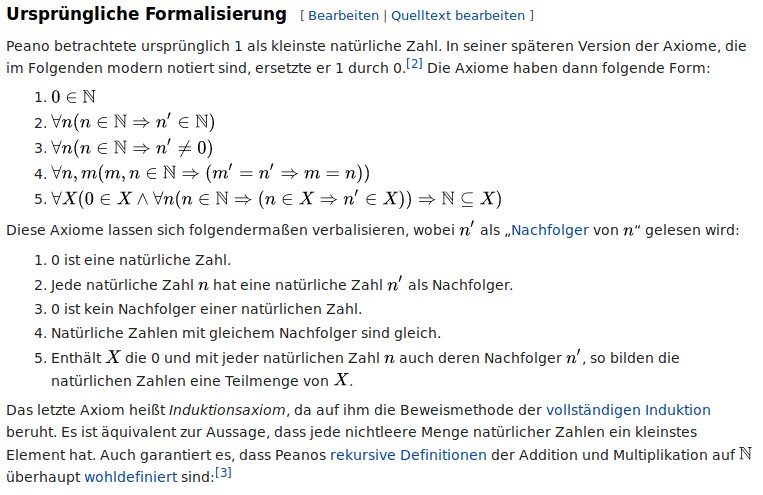
\includegraphics[scale=0.7]{vorlagen/peano.jpg} 

\subsection{Vollständige Induktion}
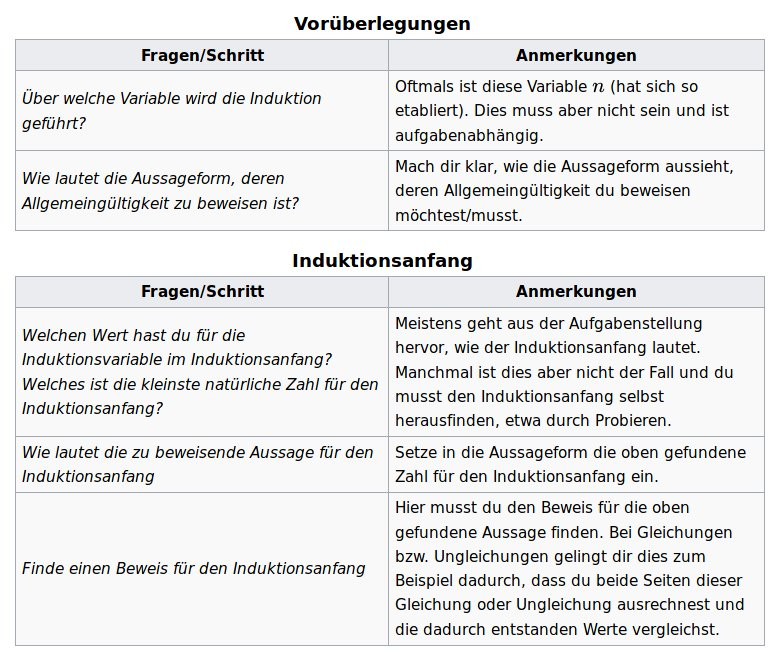
\includegraphics[scale=0.6]{vorlagen/induktion1.jpg} \\
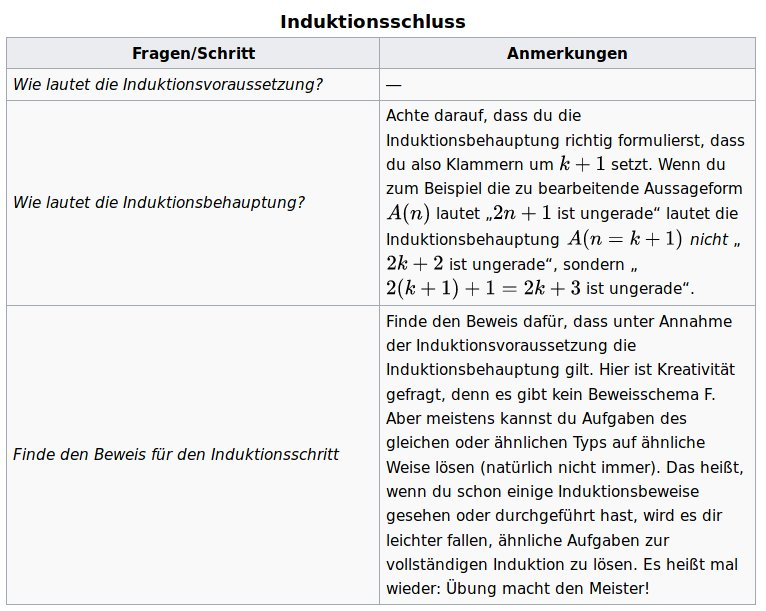
\includegraphics[scale=0.6]{vorlagen/induktion2.jpg} 
\subsubsection{Beispiel 1}
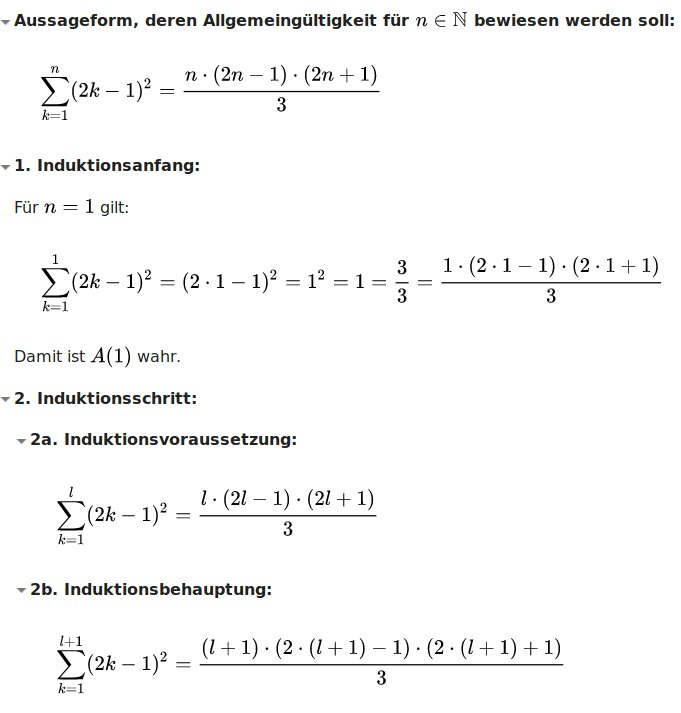
\includegraphics[scale=0.6]{vorlagen/induktion3.jpg} \newpage
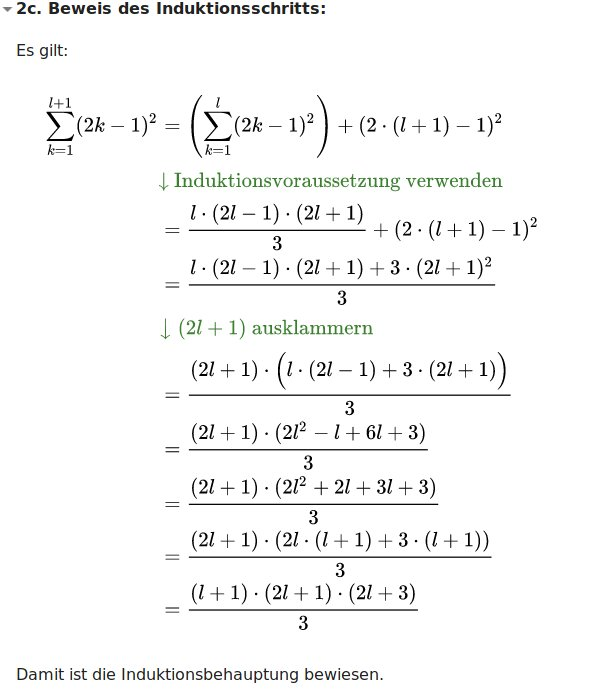
\includegraphics[scale=0.6]{vorlagen/induktion4.jpg} 
\subsubsection{Beispiel 2}
\end{document}